
\section{Experimental Results}
\label{sec:6_Expsetup}

In this section, the proposed HTL, CORAL \cite{sun2016return}, and CDTL \cite{yang2021concept}, and Melanie \cite{dong2019multistream} algorithms are compared. Three subsections are introduced: the first section focuses on the experimental setup; second, a discussion on data streams to apply all experiments on heterogeneous and homogeneous source domains, including a comparison to evaluate the runtime factor between all methods; and finally, a comparison is made between online learning and chunk-based concept drift.
\subsection{Experimental setup}
The evaluation of Heterogeneous Taxonomy Learning (HTL) involves a comparison with CORAL \cite{sun2016return}, CDTL \cite{yang2021concept}, and Melanie \cite{dong2019multistream}  which employs multiple metrics such as precision, recall, $f_1$ score \cite{sasaki2007truth}, BAC \cite{brodersen2010balanced}, and G-mean \cite{kubat1997addressing}. The experimental protocol employed for evaluation followed the test-then-train approach \cite{krawczyk2017ensemble}, where the classification model is trained on a specific data chunk and subsequently evaluated on the next chunk. The chunk size was standardized to 2000 instances. Four different classification models were used as base estimators: k-Neighbors (KNN) algorithm, Support Vector Machine (abbreviated as SVM), Gaussian Naive Bayes abbreviated as (GNB), and Hoeffding Tree (abbreviated as HT), as implemented in scikit-learn \cite{frias2014online}. We establish an ensemble classifier pool with a set limit of $L$ = 8, wherein each ensemble consists of $N$ = 4 base models. While these constraints remained fixed across all experiments, the threshold for the pool classifier in each approach was maintained at eight. Consequently, if the threshold is surpassed, the least-performing classifier is systematically eliminated. This configuration was applied consistently across all approaches to ensure fair engagement. The experiments were carried out using the Python programming language, with the source code publicly accessible on GitHub\footnote{\url{https://github.com/Amadkour/transfer_learning_with_concept_drift.git}} . When dealing with heterogeneous multisource streams, it is often impractical or not applicable to truly heterogeneous experiences. Consequently, the eigenvector technique was utilized in all related approaches. This decision stems from the fact that the algorithms in related work primarily focus on homogeneous source domains and do not address the challenges posed by heterogeneous multisource data. Therefore, heterogeneous experiments were conducted.

\subsubsection{Data Streams}
In this study, the performance of the third proposed approach was evaluated using various datasets, including synthetic data streams, a real application stream, and dataset benchmark datasets. To conduct the evaluations, the stream-learn Python library \cite{ksieniewicz2022stream,madkour2023historical} was used. As detailed in Table 1, the benchmark dataset employed in the study is the Covertype dataset. This dataset comprises 52 features, 7 classes, and a total of 581,010 instances. It serves as a standard benchmark dataset widely used in stream mining research. For the evaluation of real application streams, the Sensor Stream dataset was utilized. This dataset includes 5 features, 58 classes, and a total of 392,600 instances, representing a real-world application scenario. Synthetic datasets were generated using the scikit-learn Python package. This synthetic dataset was created to simulate data streams and evaluate the performance of the framework. The synthetic datasets consisted of 10 features and four classes and were divided into 200 chunks. Each chunk had a size of 2,000. The performance of the third proposed approach was systematically evaluated using these datasets and a stream-learn library. These evaluations provided valuable insights into the effectiveness of the framework in handling different types of data streams, including benchmark datasets, real application streams, and synthetic data streams.

\begin{table}[H]
  \centering
  \caption{Summary of Dataset Characteristics Utilized in the HTL.}
  \resizebox{\textwidth}{!}{
  \begin{tabular}{|l|c|c|c|}
  \hline
  \textbf{Dataset} & \textbf{Number of Features} & \textbf{Number of Classes} & \textbf{Number of Instances} \\ \hline
  Covertype dataset\footnote{\url{http://archive.ics.uci.edu/dataset/31/covertype}} & 40 & 7 & 581,010 \\ \hline
  Sensor Stream dataset\footnote{\url{https://www.cse.fau.edu/~xqzhu/Stream/sensor.arff}} & 5 & 58 & 392,600 \\ \hline
  Synthetic stream-52 & 52 & 5 & 200,000 \\ \hline
  Synthetic stream-8 & 8 & 4 & 200,000 \\ \hline
  \end{tabular}
  }
  \label{table:6_table1}
  \end{table}

  \subsubsection{Compared Approaches}
  In the subsequent section,the established benchmark techniques is introduced as outlined below:
  \begin{itemize}
    \item \textbf{AW-CORAL \cite{sun2016return}:} The AW- CORAL (Adaptive Weighted CORrelation ALignment) method is a simple domain adaptation technique designed to align the distributions of both source and target features without supervision. This is accomplished by aligning second-order statistics, focusing specifically on covariance, to match the distributions between the domains.
    \item \textbf{HE-CDTL \cite{sun2016return}:} The HE-CDTL approach tackles Concept Drift Transfer Learning (CDTL) by integrating knowledge from source domains and historical time steps in the target domain to improve learning performance. HE-CDTL features class-wise weighted ensemble for independent selection of historical knowledge by each class, and AW-CORAL to mitigate domain discrepancy and reduce negative knowledge transfer.
    \item \textbf{Melanie \cite{dong2019multistream}:} Multisource Online Transfer Learning for Non-stationary Environments, known as Melanie, represents the inaugural method capable of transferring knowledge across various data streaming sources in non-stationary environments. Melanie constructs numerous sub-classifiers to grasp diverse facets from distinct source and target concepts dynamically. It identifies sub-classifiers that align closely with the prevailing target concept, assembling them into an ensemble for predicting instances originating from the target concept.
  \end{itemize}

While Melanie extends online learning through chunk-based learning akin to CDTL, it exhibits two limitations: 
\begin{itemize}
  \item utilizing a global weight for each classifier, disregarding performance variation across different locations of a data chunk
  \item combining learned classifiers from these domains directly with the target classifier, which may impede effective knowledge transfer due to domain discrepancies. Hence, the third proposed approach (HTL) is compared with AW- CORAL \cite{sun2016return} and HE-CDTL \cite{yang2021concept}.
\end{itemize}

\subsection{Analysis of Experimental Results}

This section evaluates the proposed approach's performance across multiple data streams using five metrics: $f_1$ score, precision, recall, G-mean, and BAG. Two visualization techniques, radar and line diagrams, were employed. Radar charts summarized algorithm performance across metrics, while line diagrams focused on G-mean comparisons across 100 chunks. The first five experiments used line diagrams, and the last two combined radar and line charts, offering a detailed evaluation of the third proposed approach under diverse scenarios.

\subsubsection{Results on Target Domains Dataset without Source Domain}
Figure \ref{fig:6_exp1} presents the results of applying various classification methods to the Covertype dataset without employing a source domain stream. The line diagram reveals the classification performance, assessed using the G-mean metric, over 100 data chunks for each method. Philosophically, the observed trajectory of performance reflects an epistemological journey from initial uncertainty to eventual refinement and adaptation. The suboptimal performance during the initial 10 chunks suggests a nascent phase where the system's understanding is limited, akin to the formative stages of knowledge acquisition. This phase is marked by an incomplete pool of classifiers, signifying the constraints of limited epistemic resources. As the classifier pool expands, representing an enrichment of the system’s cognitive tools, the DES technique demonstrates an enhanced ability to discern and apply the most suitable classifier for each incoming data chunk. This mirrors the philosophical principle of cumulative epistemic progress, where successive integration of knowledge resources fosters improved understanding and capability. Between chunk 20 and the final chunk, HTL consistently outperforms other methods. This superiority is attributable to its weighting mechanism, which assigns significance to historical classifiers, embodying a philosophical stance that values historical precedent and contextual relevance in constructing present knowledge. The ability of HTL to effectively leverage this weighting method facilitates the training of the classifier pool, thereby amplifying its overall efficacy.  
In contrast, the variable performance of CORAL and CDTL in certain chunks highlights the inherent challenges of reconciling differing approaches to knowledge adaptation. This variability underscores the dynamic interplay of methodologies, each striving to balance generality and specificity in their engagement with a continually evolving data stream.
\begin{figure}[H]
	\centering
	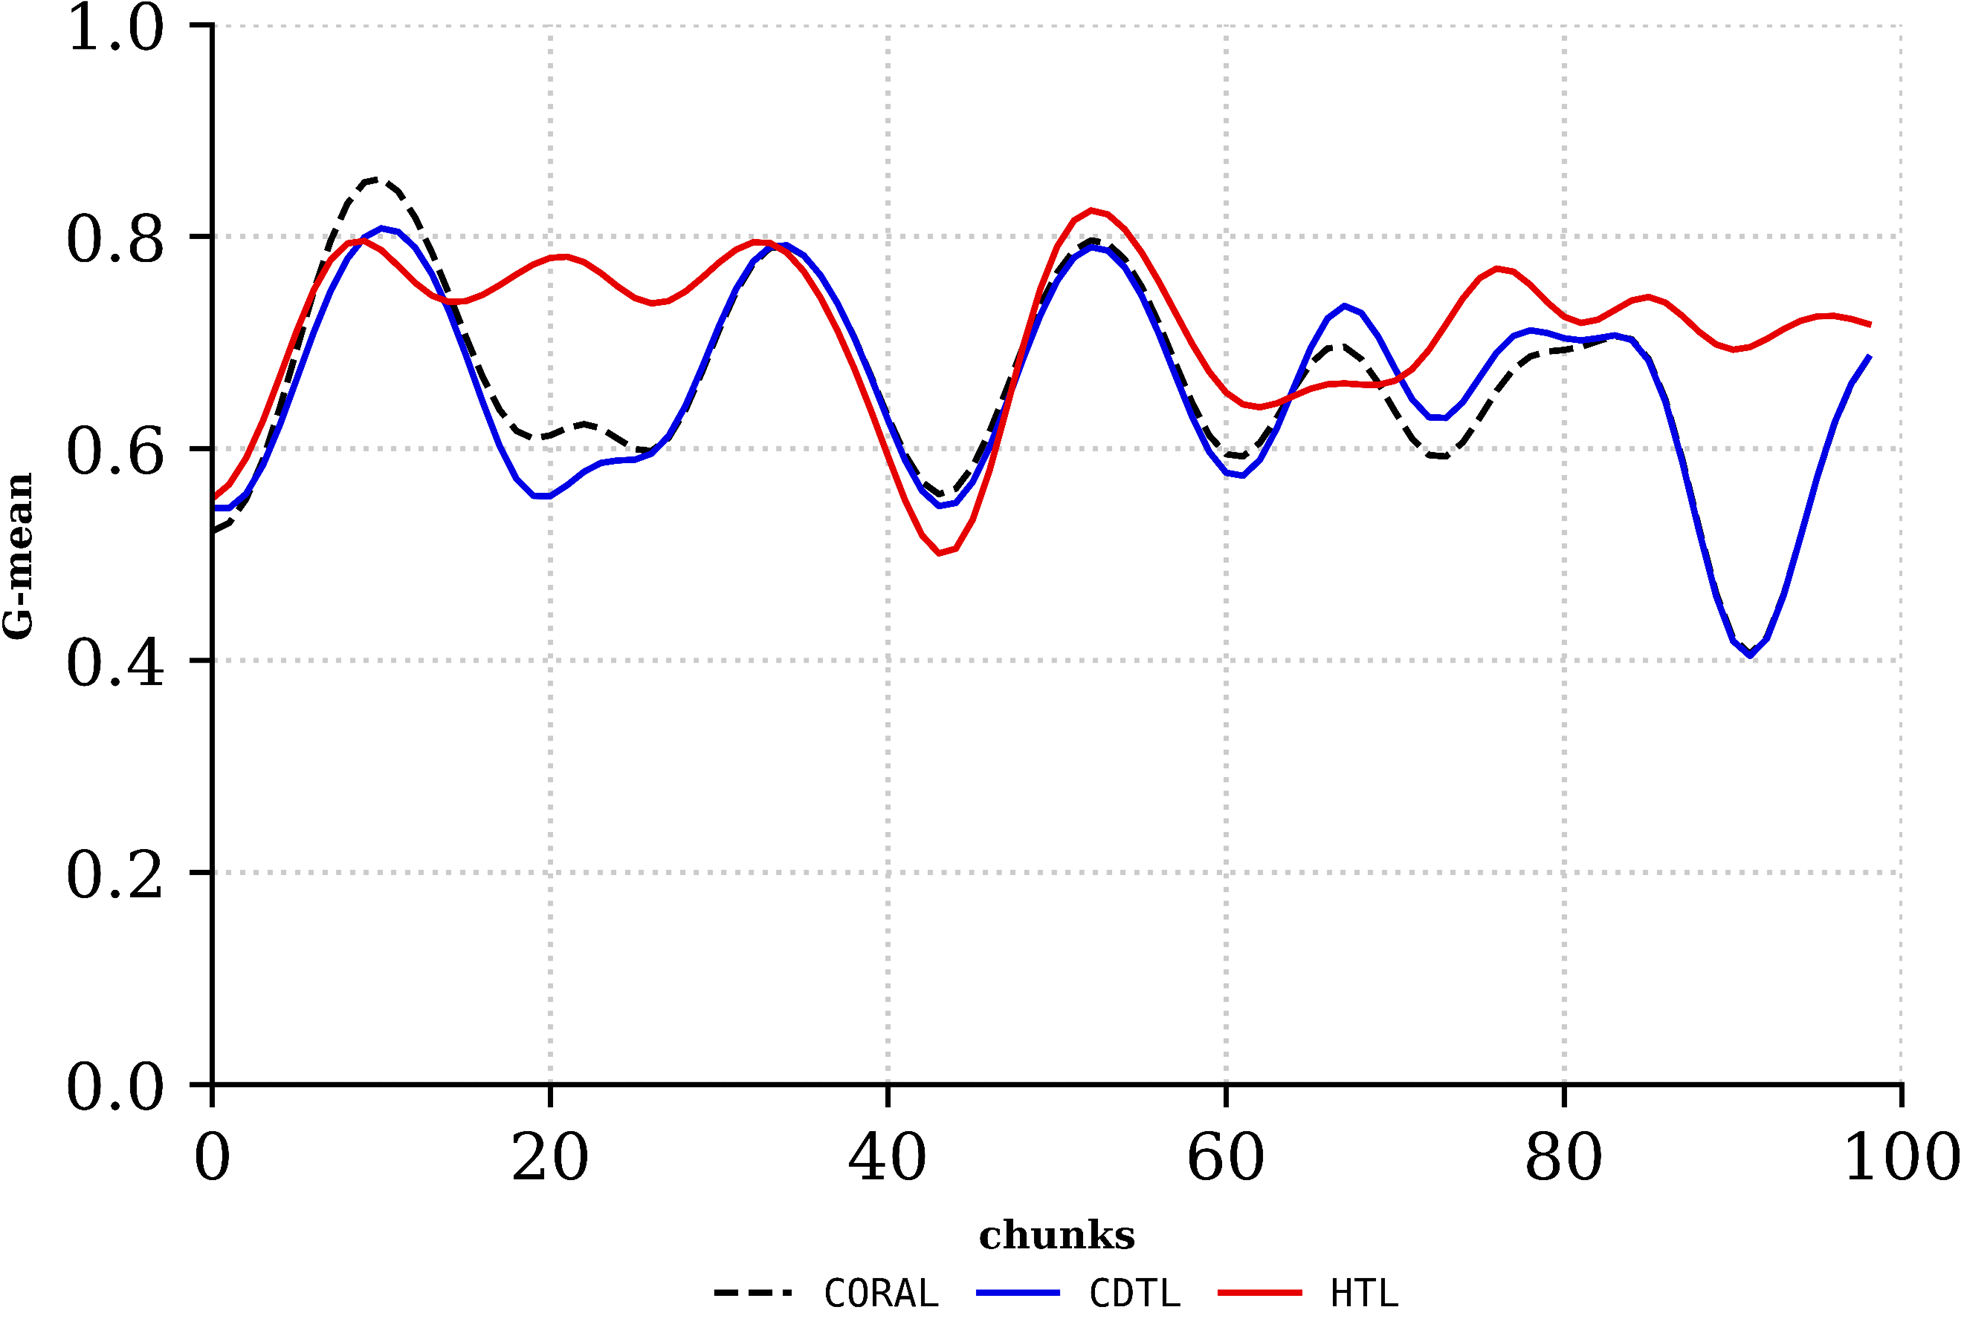
\includegraphics[width=0.6\linewidth]{6_transfer_learning/figures/exp1_0.png}
  \caption{Results of the Covertype Stream as the Target Domain without the Source Domain.}

	\label{fig:6_exp1}
\end{figure}
\begin{figure}[H]
	\centering
	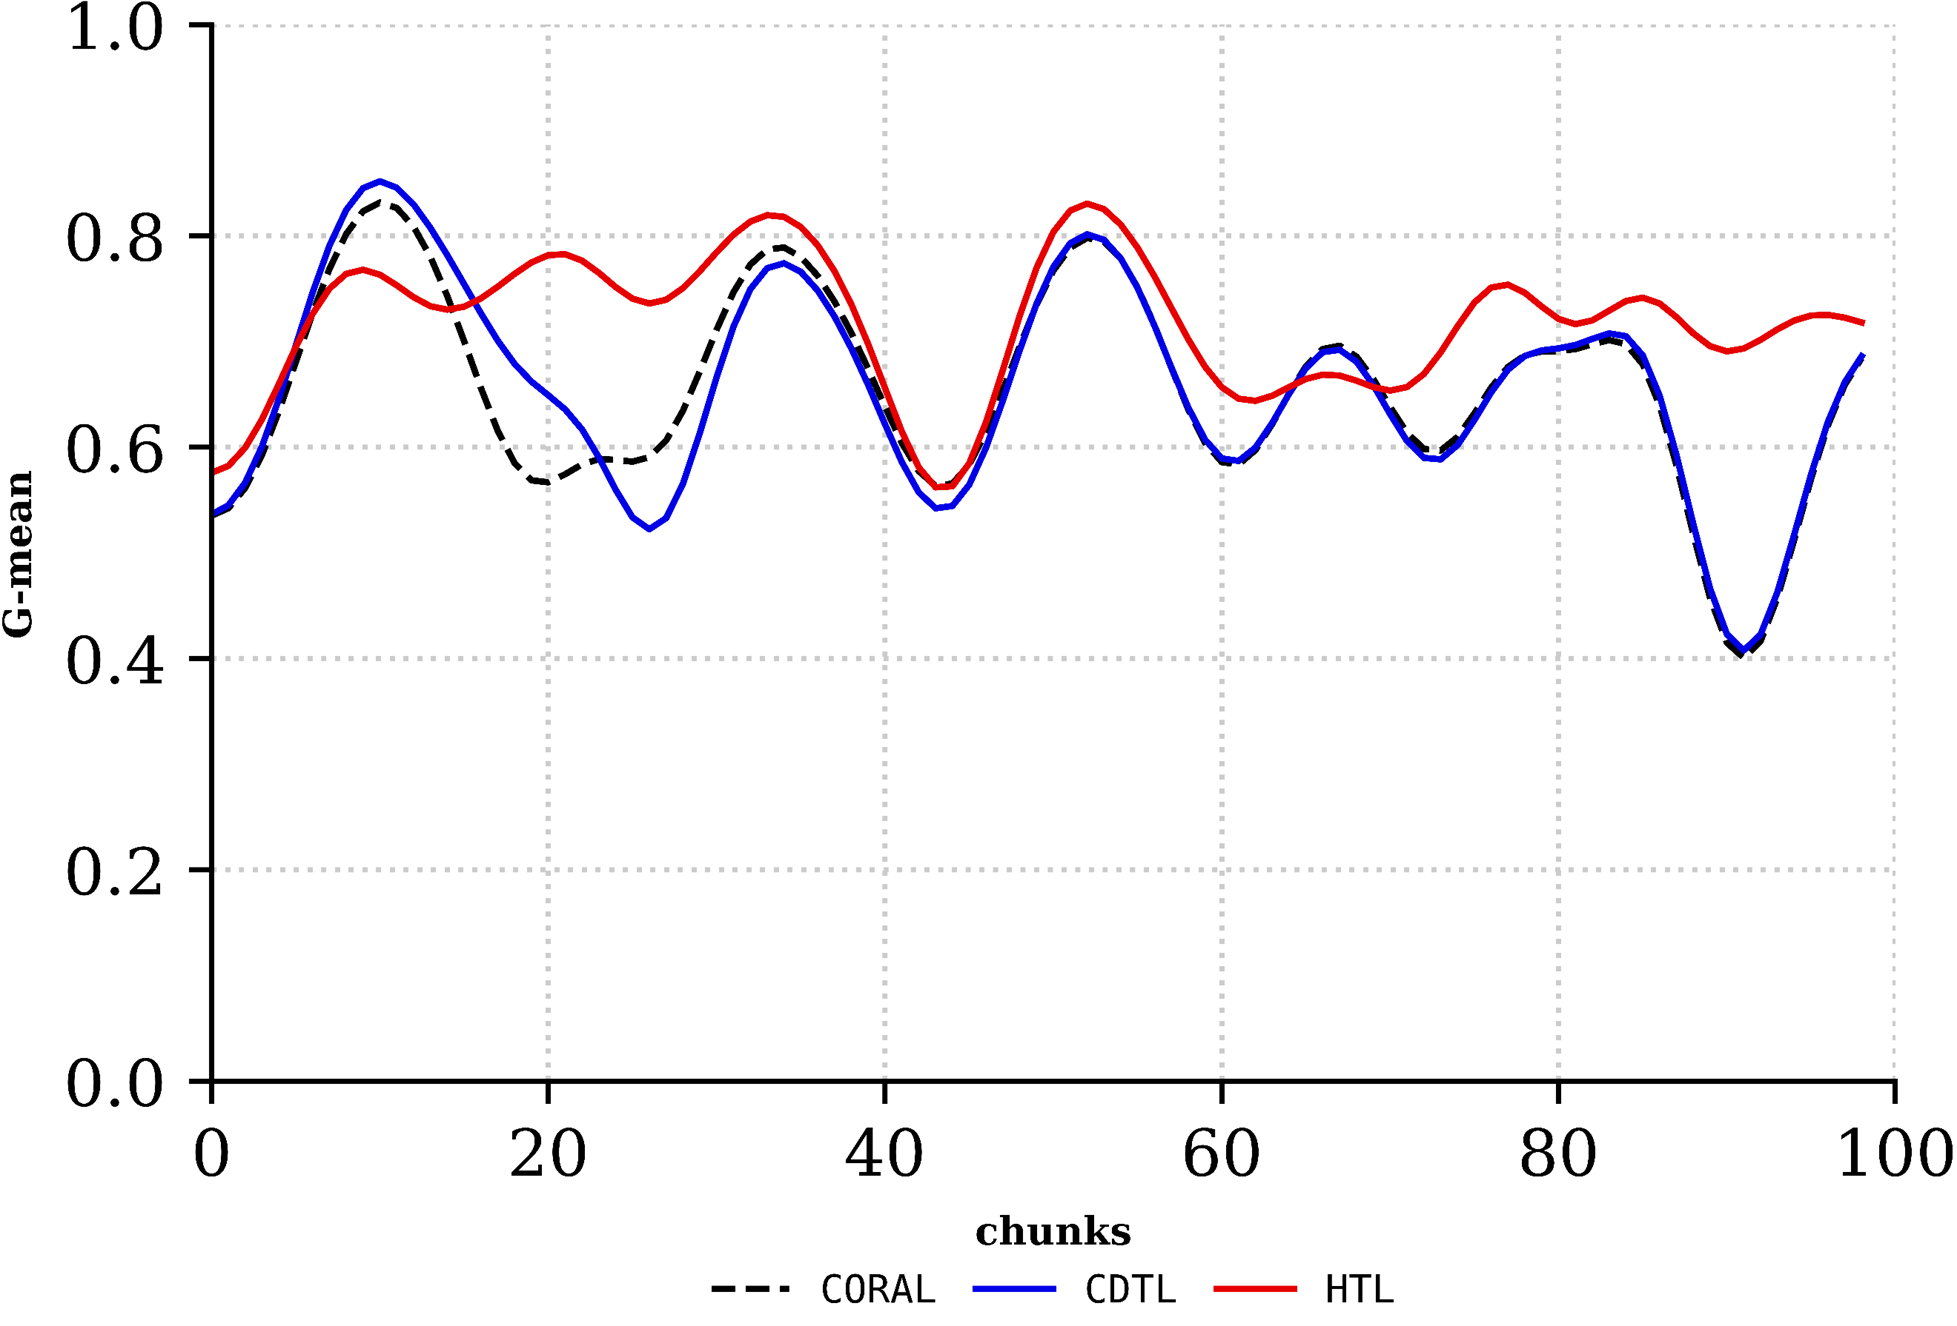
\includegraphics[width=0.6\linewidth]{6_transfer_learning/figures/exp1_1.png}
	\caption{Performance results of the Covertype Stream as the target domain using homogeneous source domains.}

	\label{fig:6_exp2}
\end{figure}

\subsubsection{Results on the Homogeneous Source Domains Dataset}
Figure \ref{fig:6_exp2} illustrates the outcomes of applying the compared methods to the Covertype data stream as a target domain, with Synthetic-52 serving as a homogenous source domain. This scenario introduces an epistemological dimension rooted in the interaction between prior knowledge (the source domain) and newly encountered contexts (the target domain). The line diagram reveals HTL’s initially suboptimal performance across the first eight chunks, attributable to the limited pool of classifiers available in the early phase. This aligns with the philosophical notion of an incomplete epistemic framework, where insufficient resources impede initial understanding. As the classifier pool expands beyond the eighth chunk, HTL’s performance improves, underscoring the significance of cumulative resource enrichment in advancing predictive accuracy. CDTL maintains consistent performance throughout the chunks, reflecting an equilibrium-based adaptation strategy that prioritizes stability over dynamic optimization. Meanwhile, CORAL’s consistently lower performance highlights the potential limitations of certain methodologies in transferring knowledge effectively across domains, pointing to the philosophical challenge of achieving universality in adaptive systems.  

Notably, HTL achieves the highest performance across all chunks, emphasizing the utility of its weighting mechanism and its capacity to harness the source domain knowledge effectively. The superior performance of both CDTL and HTL in Figure \ref{fig:6_exp2} compared to Figure \ref{fig:6_exp1} reflects the epistemological advantage conferred by incorporating Synthetic-52 as a source domain. This source-target synergy illustrates the philosophical principle of grounded learning, where external, homogenous knowledge sources enhance the capacity to navigate and adapt to complex, evolving data streams.  

The contrasting scenarios in Figures \ref{fig:6_exp1} and \ref{fig:6_exp2} underscore the critical role of prior knowledge in shaping learning trajectories. In the absence of a source domain, as in Figure \ref{fig:6_exp1}, the methods must independently construct their epistemic framework, leading to comparatively constrained performance. Conversely, the inclusion of a source domain, as shown in Figure \ref{fig:6_exp2}, facilitates a richer epistemic interplay, enhancing adaptability and robustness in the face of dynamic data challenges.


\subsubsection{Results on One Heterogeneous Source Domain}
\begin{figure}[H]
	\centering
	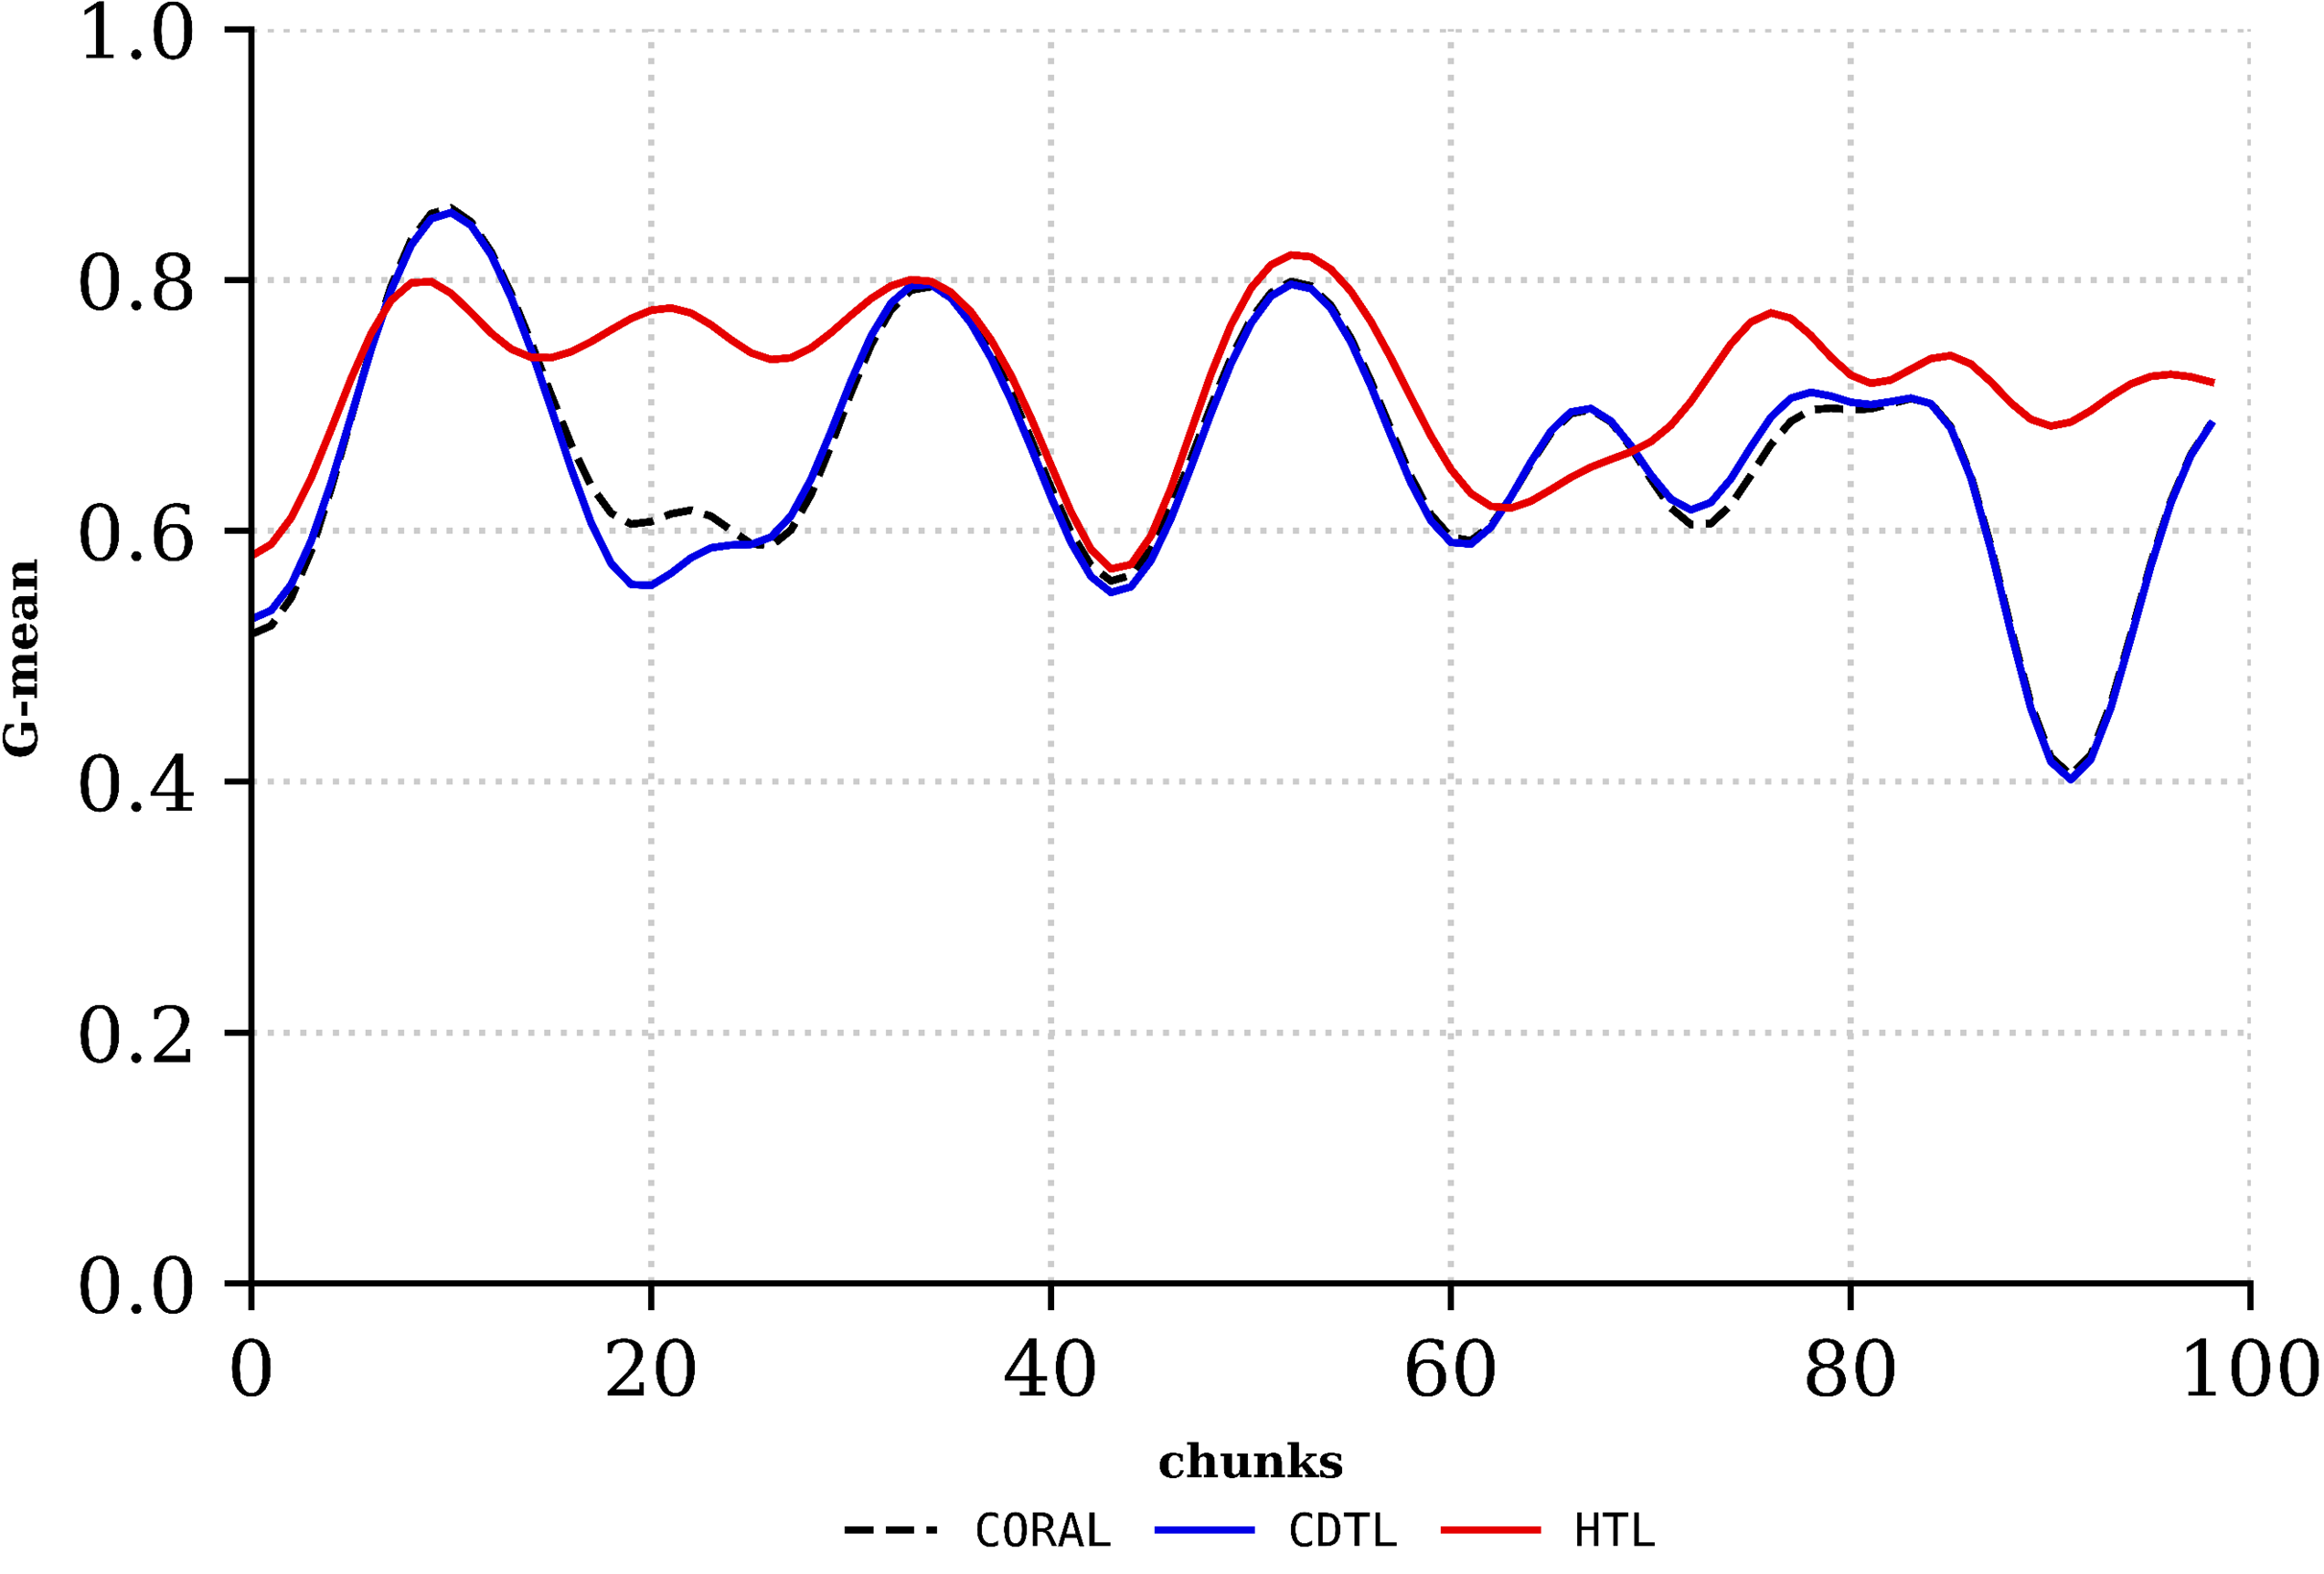
\includegraphics[width=0.6\linewidth]{6_transfer_learning/figures/exp2_0.png}
  \caption{Performance results of the Covertype Stream as the target domain with a single heterogeneous source domain.}

	\label{fig:6_exp3}
\end{figure}
Figure \ref{fig:6_exp3} presents the results of applying the compared methods to the Covertype data stream as the target domain, with Synthetic-8 as a heterogeneous source domain. This experiment explores the epistemological dynamics of knowledge transfer across domains with differing structures, reflecting the philosophical challenges of reconciling heterogeneity in adaptive systems. The Synthetic-8 stream, with its distinct dimensionality (eight features and four classes), contrasts with the Covertype stream. While HTL is inherently designed to handle heterogeneous sources, specific adjustments, such as the application of the eigenvector technique, were required to enable CORAL and CDTL to operate within this domain. This adaptation highlights the importance of methodological flexibility in addressing epistemic diversity and bridging structural disparities between domains.  
The line diagram demonstrates variability in the performance of the approaches across chunks, suggesting that the contribution of the source domain's knowledge is contingent on its alignment with the target domain’s requirements. HTL consistently achieves superior performance across almost all chunks, emphasizing its robust capacity for extracting and applying positive knowledge from heterogeneous sources. This superior adaptability reflects a philosophical commitment to leveraging epistemic pluralism, where diverse knowledge sources enrich the learning system’s overall efficacy.  

In contrast, the comparatively lower performance of CORAL and CDTL underscores the inherent challenges these methods face when transferring knowledge across domains with significant structural differences. The need for eigenvector-based adjustments further emphasizes their limited native capacity for heterogeneous adaptation, revealing the philosophical tension between static methodologies and dynamic, cross-domain requirements. This experiment exemplifies the critical role of epistemological adaptability in heterogeneous environments. The consistent success of HTL underscores the potential of methodologies that embrace diversity in knowledge sources, whereas the relative struggles of CORAL and CDTL highlight the constraints of approaches rooted in homogeneity.

\subsubsection{Results on All Heterogeneous and Covertype as the Target Domain}
\begin{figure}[H]
	\centering
	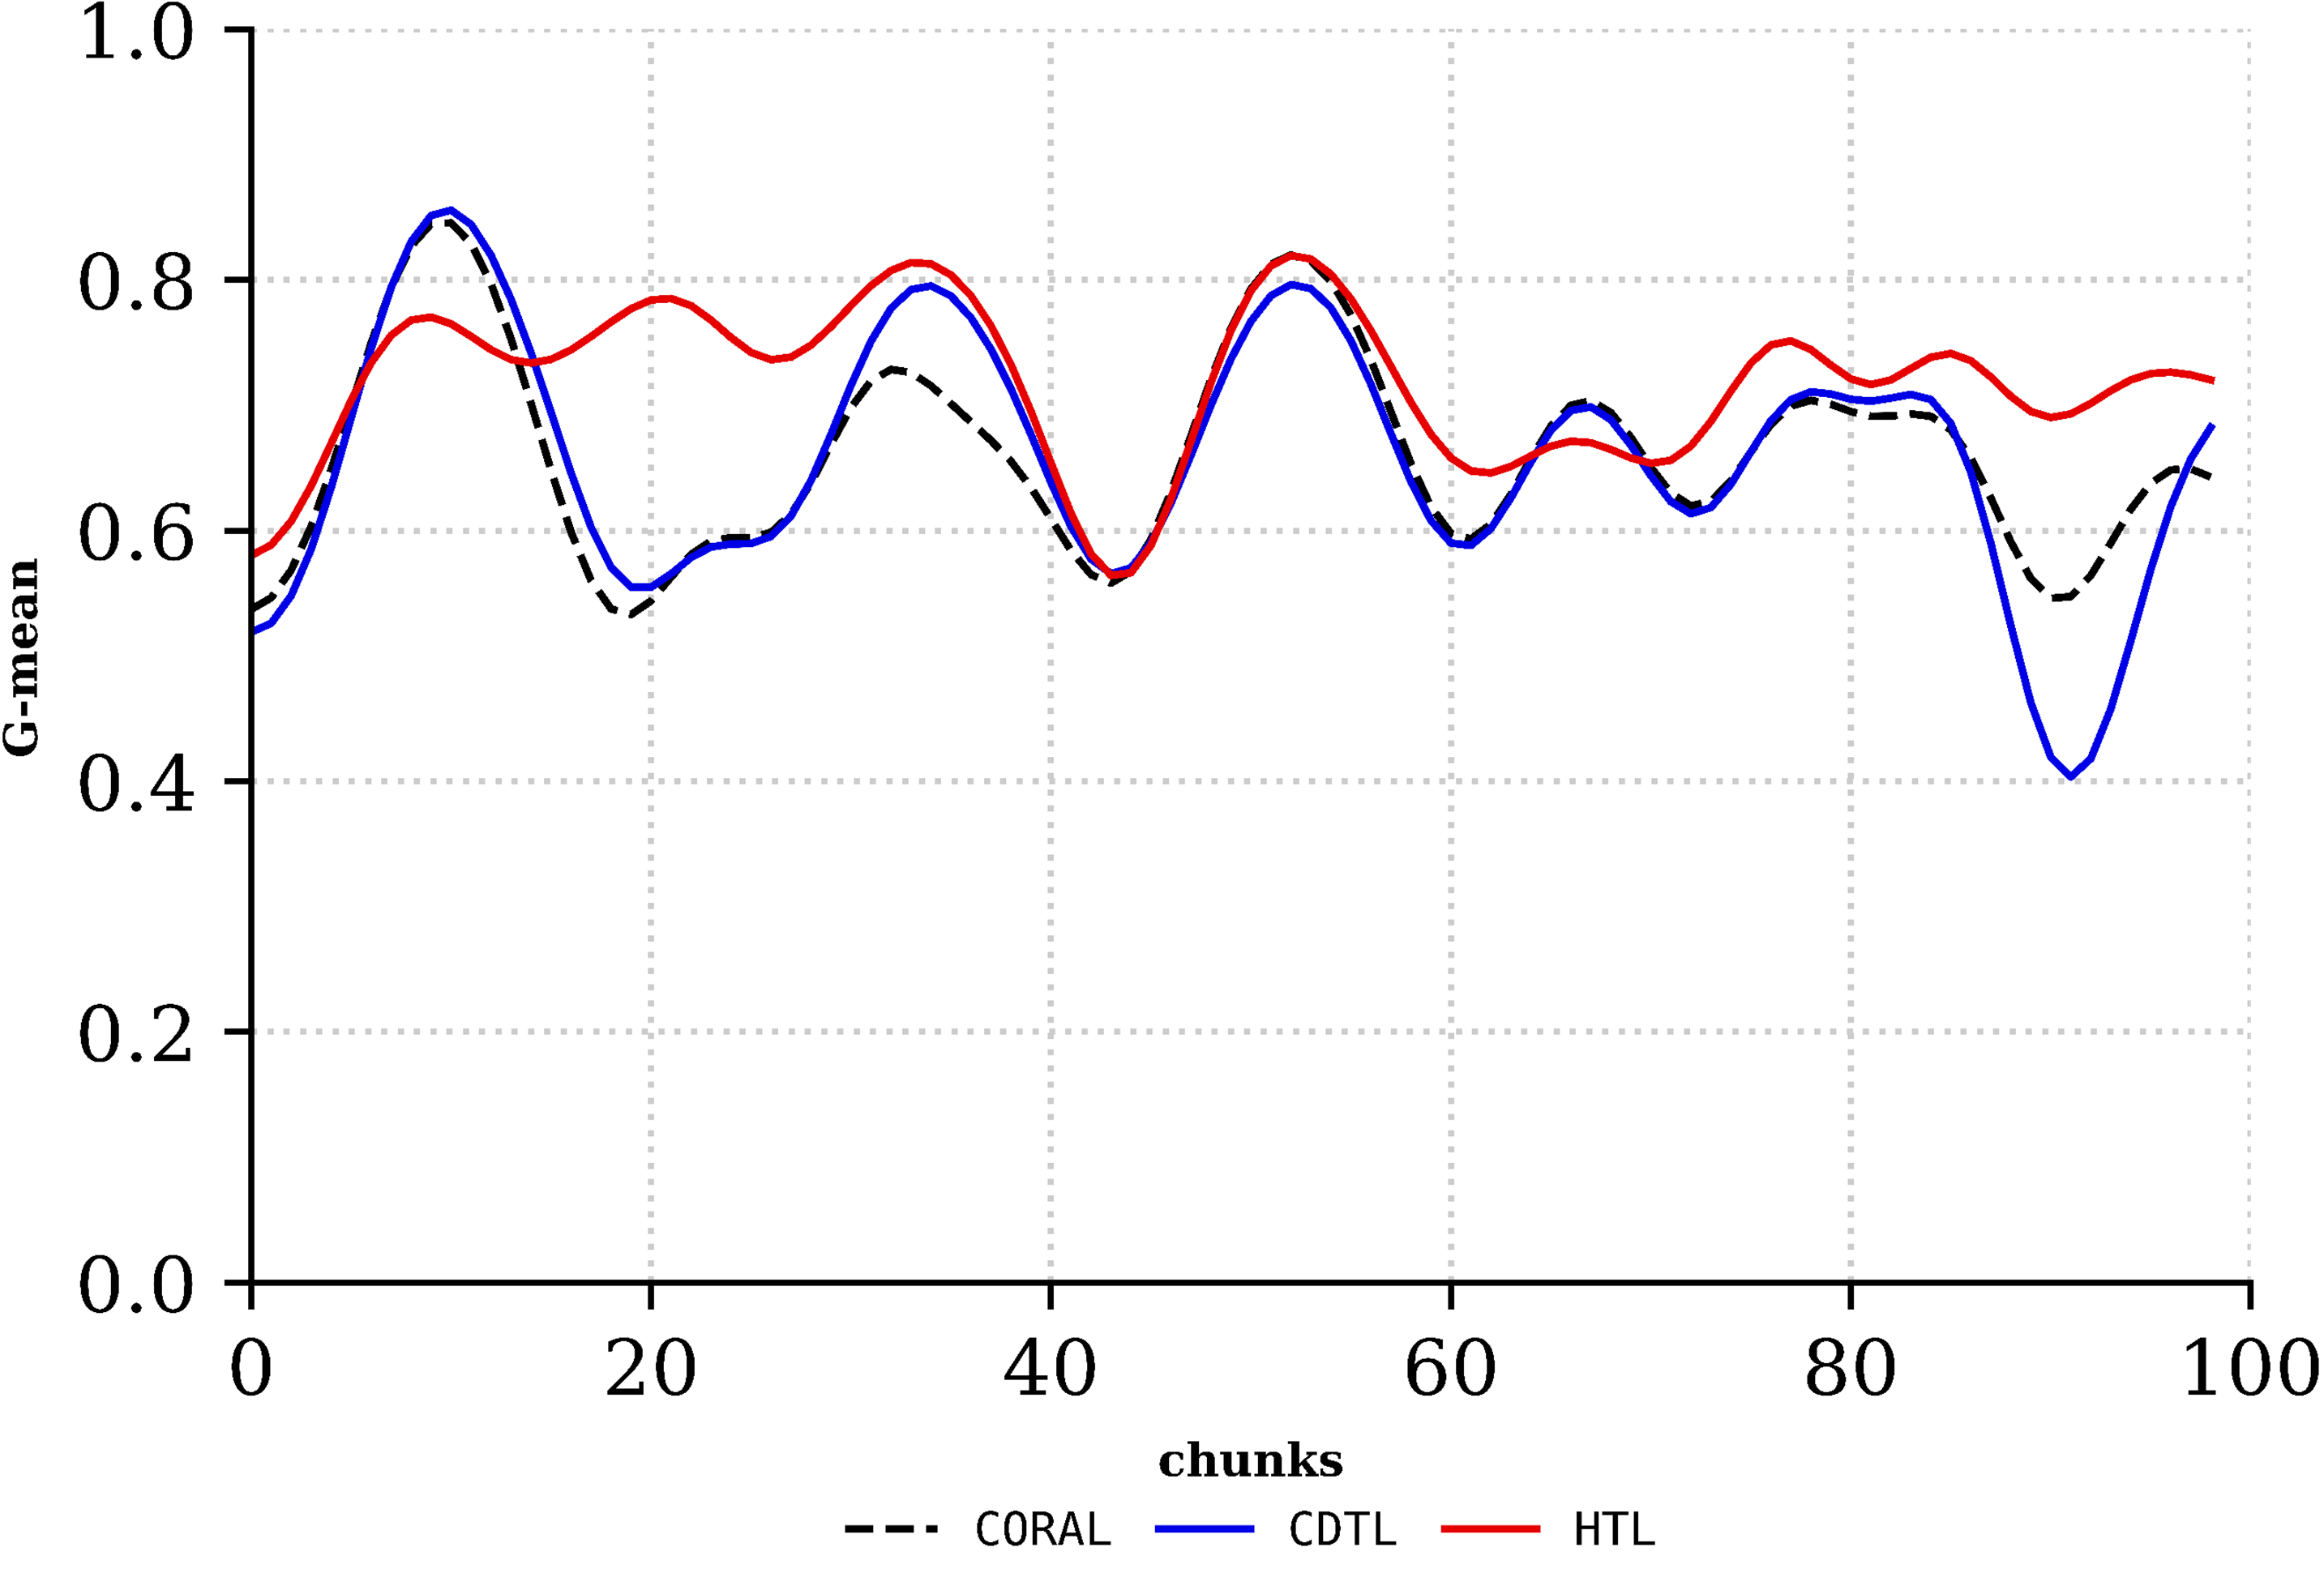
\includegraphics[width=0.6\linewidth]{6_transfer_learning/figures/exp2_1.png}
  \caption{Performance results of the Covertype Stream as the target domain with multiple heterogeneous source domains.}
	\label{fig:6_exp4}
\end{figure}
Figures \ref{fig:6_exp4} and \ref{fig:6_exp5} delve into the impact of incorporating multiple heterogeneous source domains on the classification performance of various methods, offering a nuanced philosophical reflection on the interplay between diversity, adaptability, and resilience in dynamic environments. In Figure \ref{fig:6_exp4}, the Covertype data stream serves as the target domain, while Synthetic-8, Synthetic-52, and Sensor streams act as heterogeneous source domains. The results demonstrate a notable improvement over previous experiments, underscoring the epistemic value of increasing the number of source domains. This enhancement reflects the philosophical principle of cumulative epistemic diversity: as the pool of source domains expands, the system gains access to a broader spectrum of positive knowledge. Each additional domain contributes incrementally to the refinement of classifiers, facilitating more accurate and adaptive performance.

Figure \ref{fig:6_exp5}, employing the same experimental setup but switching the target domain to the Sensor stream, highlights the influence of contextual factors on performance. The Sensor stream introduces higher noise levels and frequent concept drifts, presenting significant challenges to all methods. Despite these adversities, HTL consistently achieves superior performance across all chunks, reinforcing its adaptability and capacity to navigate complex and unstable environments. This robustness aligns with a philosophical framework that values resilience and context-sensitive adaptation in epistemic systems. In contrast, CORAL and CDTL exhibit nearly identical performance values across most chunks, indicating a more static approach to adaptation. Their inability to capitalize fully on the heterogeneity of source domains or mitigate the challenges posed by the Sensor stream underscores the philosophical tension between generality and specificity in dynamic learning systems. While they may perform adequately in stable or homogenous contexts, their relative rigidity limits their efficacy in environments marked by noise and drift.
\begin{figure}[H]
	\centering
	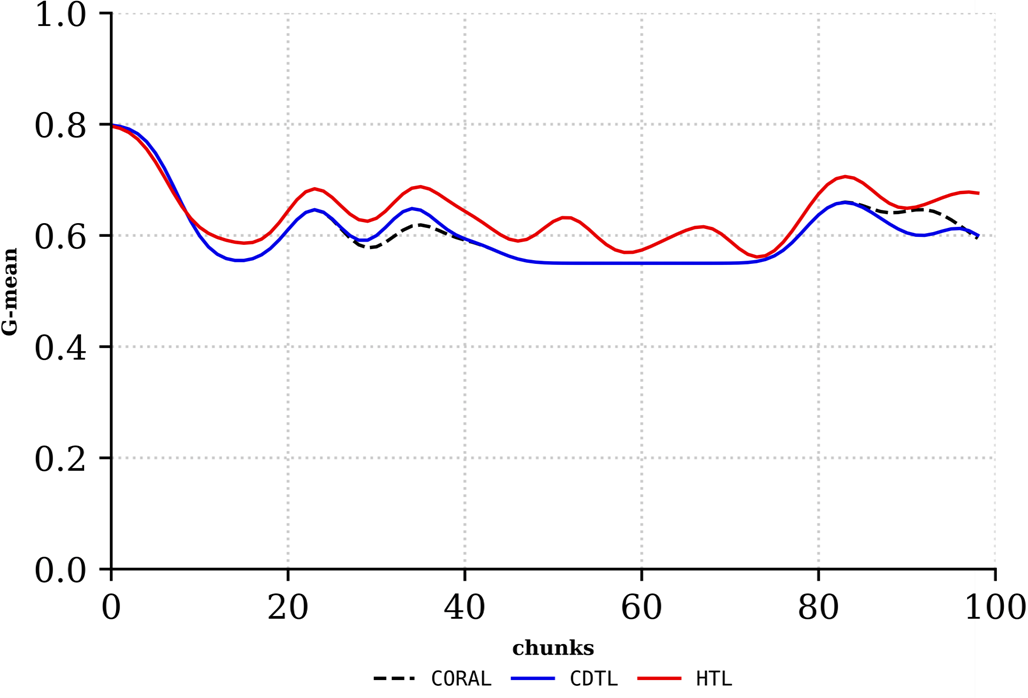
\includegraphics[width=0.6\linewidth]{6_transfer_learning/figures/exp3.png}
  \caption{Results of the Sensor Stream as the Target Domain with Multiple Heterogeneous Source Domains.}

	\label{fig:6_exp5}
\end{figure}

\subsubsection{Results on One Heterogeneous Source Domain}
This section evaluates the overall performances of CORAL, CDTL, and HTL across five performance metrics: $f_1$ score, precision, recall, G-mean, and BAG. Table \ref{table:6_table2} summarizes the average performance across 100 data chunks for each method and highlights HTL's consistent superiority in most configurations.

In the first experiment, which lacked a source domain, CORAL achieved the highest precision, while HTL excelled across the other metrics. In subsequent experiments, HTL consistently outperformed other methods in most metrics, except for recall in the third experiment, where CDTL achieved the best results. The performance improvement across experiments reflects the incremental addition of source domains, which enhances the positive knowledge available to the classifiers, thereby improving overall performance.
  
\begin{table}[H]
  \centering
  \caption{Comprehensive performance comparison of CORAL, CDTL, and HTL across all previous experiments.}
  \resizebox{\textwidth}{!}{
  \begin{tabular}{|l|l|c|c|c|}
  \hline
  \textbf{Experiment}                            & \textbf{Metric} & \textbf{CORAL} & \textbf{CDTL} & \textbf{HTL} \\ \hline
  \multirow{4}{*}{Without source domain}         & BAC             & 0.723          & 0.723         & \textbf{0.725} \\ \cline{2-5} 
                                                 & G-mean          & 0.652          & 0.654         & \textbf{0.717} \\ \cline{2-5} 
                                                 & $f_1$ score        & 0.875          & 0.874         & \textbf{0.890} \\ \cline{2-5} 
                                                 & Precision       & 0.827          & 0.823         & \textbf{0.851} \\ \cline{2-5} 
                                                 & Recall          & \textbf{0.950} & 0.944         & 0.939          \\ \hline
  \multirow{4}{*}{Homogenous source domain}      & BAC             & 0.731          & 0.730         & \textbf{0.755} \\ \cline{2-5} 
                                                 & G-mean          & 0.658          & 0.653         & \textbf{0.717} \\ \cline{2-5} 
                                                 & $f_1$ score        & 0.876          & 0.875         & \textbf{0.858} \\ \cline{2-5} 
                                                 & Precision       & 0.830          & 0.829         & \textbf{0.851} \\ \cline{2-5} 
                                                 & Recall          & 0.950          & 0.950         & \textbf{0.953} \\ \hline
  \multirow{4}{*}{Single heterogeneous source domain} & BAC         & 0.732          & 0.732         & \textbf{0.757} \\ \cline{2-5} 
                                                 & G-mean          & 0.661          & 0.657         & \textbf{0.717} \\ \cline{2-5} 
                                                 & $f_1$ score        & 0.875          & 0.875         & \textbf{0.859} \\ \cline{2-5} 
                                                 & Precision       & 0.835          & 0.835         & \textbf{0.851} \\ \cline{2-5} 
                                                 & Recall          & 0.947          & 0.950         & \textbf{0.953} \\ \hline
  \multirow{4}{*}{Multisource heterogeneous domain (Covertype stream)} & BAC & 0.732  & 0.732         & \textbf{0.757} \\ \cline{2-5} 
                                                 & G-mean          & 0.661          & 0.661         & \textbf{0.717} \\ \cline{2-5} 
                                                 & $f_1$ score        & 0.875          & 0.875         & \textbf{0.859} \\ \cline{2-5} 
                                                 & Precision       & 0.835          & 0.835         & \textbf{0.851} \\ \cline{2-5} 
                                                 & Recall          & 0.947          & 0.950         & \textbf{0.953} \\ \hline
  \multirow{4}{*}{Multisource heterogeneous domain (Sensor stream)} & BAC & 0.998  & 0.998         & \textbf{0.998} \\ \cline{2-5} 
                                                 & G-mean          & 0.971          & 0.971         & \textbf{0.992} \\ \cline{2-5} 
                                                 & $f_1$ score        & 0.997          & 0.997         & \textbf{0.997} \\ \cline{2-5} 
                                                 & Precision       & 0.998          & 0.998         & \textbf{0.998} \\ \cline{2-5} 
                                                 & Recall          & 0.998          & 0.998         & \textbf{0.998} \\ \hline
  \end{tabular}
  }

  \label{table:6_table2}
  \end{table}

\subsection{Analysis Runtime between CORAL, CDTL, and HTL Techniques}
From a philosophical perspective, the experimental results underscore the nuanced interplay between technological efficiency and contextual suitability in heterogeneous transfer learning. The choice of an optimal algorithm emerges not as an absolute truth but as a contextual decision shaped by the characteristics of the dataset and the temporal demands of the application. The study’s findings illuminate the inherent efficiency of the HTL algorithm, particularly in scenarios demanding rapid iteration. For instance, the HTL algorithm's completion of 100 iterations within 304 seconds in the homogeneous source domain setting starkly contrasts with the prolonged runtimes of CORAL and CDTL algorithms. This efficiency is not merely a quantitative advantage but symbolizes the evolving imperative of time-conscious adaptability in machine learning \cite{ref}. The philosophical significance deepens when considering the diverse source domain configurations—homogeneous, absent, single heterogeneous, and multi-source heterogeneous—each representing varying degrees of complexity and unpredictability. The HTL algorithm's consistent efficiency across these scenarios reflects a harmonious balance between universality and specificity. It challenges the idea of algorithmic rigidity, suggesting that adaptability and context-awareness are the cornerstones of effective machine learning paradigms \cite{ref}. Thus, the findings, accentuated by the runtime data in Table \ref{table:6_table3}, reveal the HTL algorithm as not merely a technical tool but a conceptual embodiment of efficiency tailored to the exigencies of dynamic, real-world applications. In this light, its superiority is not only functional but philosophical, aligning with the broader pursuit of practical excellence in algorithmic design and implementation.
\begin{table}[H]
  \centering
  \caption{Runtimes (in seconds) for CORAL, CDTL, and HTL.}
  \resizebox{\textwidth}{!}{
  \begin{tabular}{|l|l|l|c|c|c|}
  \hline
  \textbf{Experience}                              & \textbf{Target domain} & \textbf{Source Domain}                      & \textbf{CORAL} & \textbf{CDTL} & \textbf{HTL} \\ \hline
  without source domain                            & Covertype              & None                                         & 312            & 312           & \textbf{304} \\ \hline
  Homogenous source domain                         & Covertype              & Synthetic-52                                 & 6165           & 614           & \textbf{606} \\ \hline
  Single heterogeneous source domain               & Covertype              & Synthetic-8                                  & 6060           & 4703          & \textbf{4475} \\ \hline
  Multi-source heterogeneous domain                & Covertype              & Sensor, Synthetic-52, and Synthetic-8        & 23011          & 14043         & \textbf{13824} \\ \hline
  Multi-source heterogeneous domain                & Sensor                 & Covertype, Synthetic-52, and Synthetic-8     & 14524          & 3052          & \textbf{3005} \\ \hline
  \end{tabular}
  }
  \label{table:6_table3}
  \end{table}
  
\subsection{Analysis performance and runtime of HTL for online learning and chunk-based concept drift}

This experiment explores the temporal dynamics of various learning techniques, comparing the efficiency of online learning with chunk-based concept drift methods. The time savings provided by drift detectors like EDDM and ADWIN offer insights into the relationship between learning time and performance. The EDDM drift detector is notably efficient, detecting 40 drifted chunks out of 100, which highlights a pragmatic approach to reducing computational overhead while maintaining accuracy. This efficiency aligns with the concept of "pragmatic optimization," aiming to balance time and performance within real-world constraints \cite{ref}. In contrast, the ADWIN drift detector, which detects 63 drifted chunks and requires 63 learning times, demonstrates a trade-off between improved drift detection and time efficiency. This suggests that optimal performance is often context-dependent, with the most efficient algorithm not necessarily being the one that minimizes time, but one that balances all relevant factors. On the other hand, online learning, requiring 100 learning times for 100 chunks, proves to be the least time-efficient. However, its design may reflect a commitment to consistency and robustness, even at the expense of time.
Figures \ref{fig:6_exp6} and \ref{fig:6_exp7}, which include radar and line diagrams, visually capture the tension between time efficiency and performance. While online learning achieves optimal performance, its higher time consumption highlights the conflict between pursuing perfection and managing resource limitations. This analysis emphasizes that efficiency is not solely about minimizing time but involves balancing multiple factors in real-world applications.
\begin{figure}[H]
	\centering
	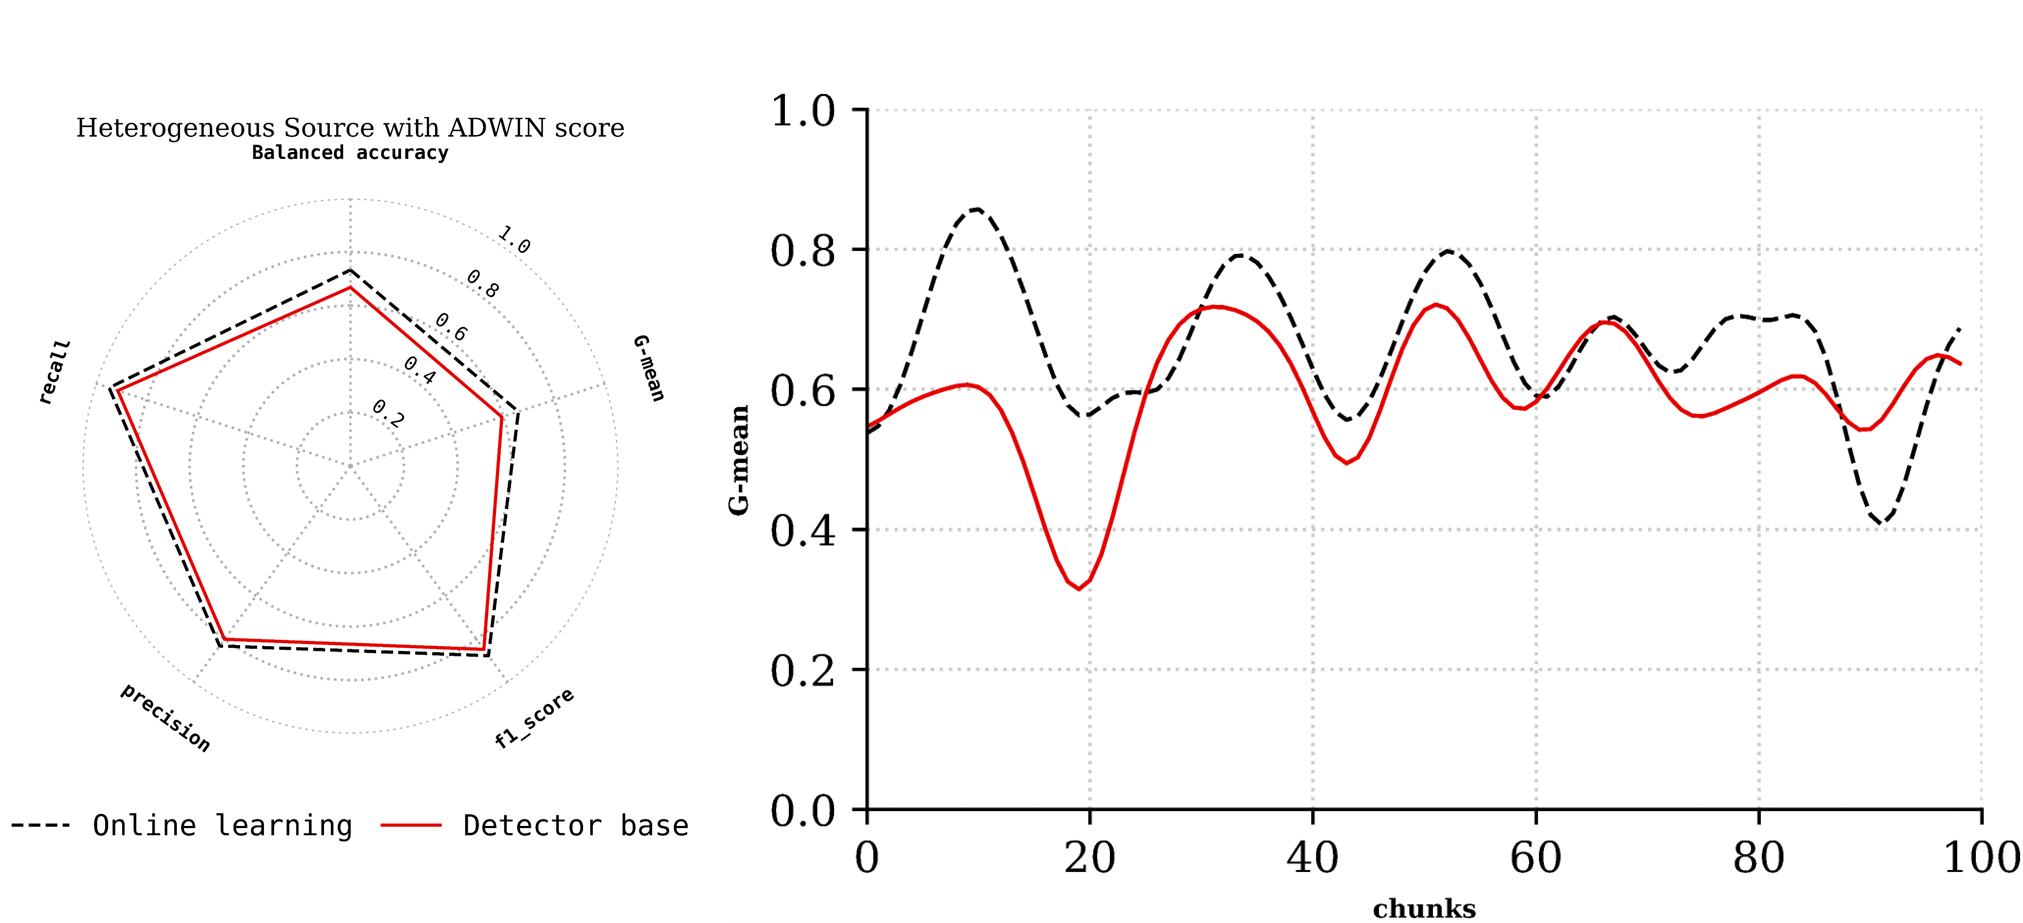
\includegraphics[width=1\linewidth]{6_transfer_learning/figures/exp4.png}
	\caption{Online learning and chunk-based results for the Covertype stream using the ADWIN detector.}
	\label{fig:6_exp6}
\end{figure}

\begin{figure}[H]
	\centering
	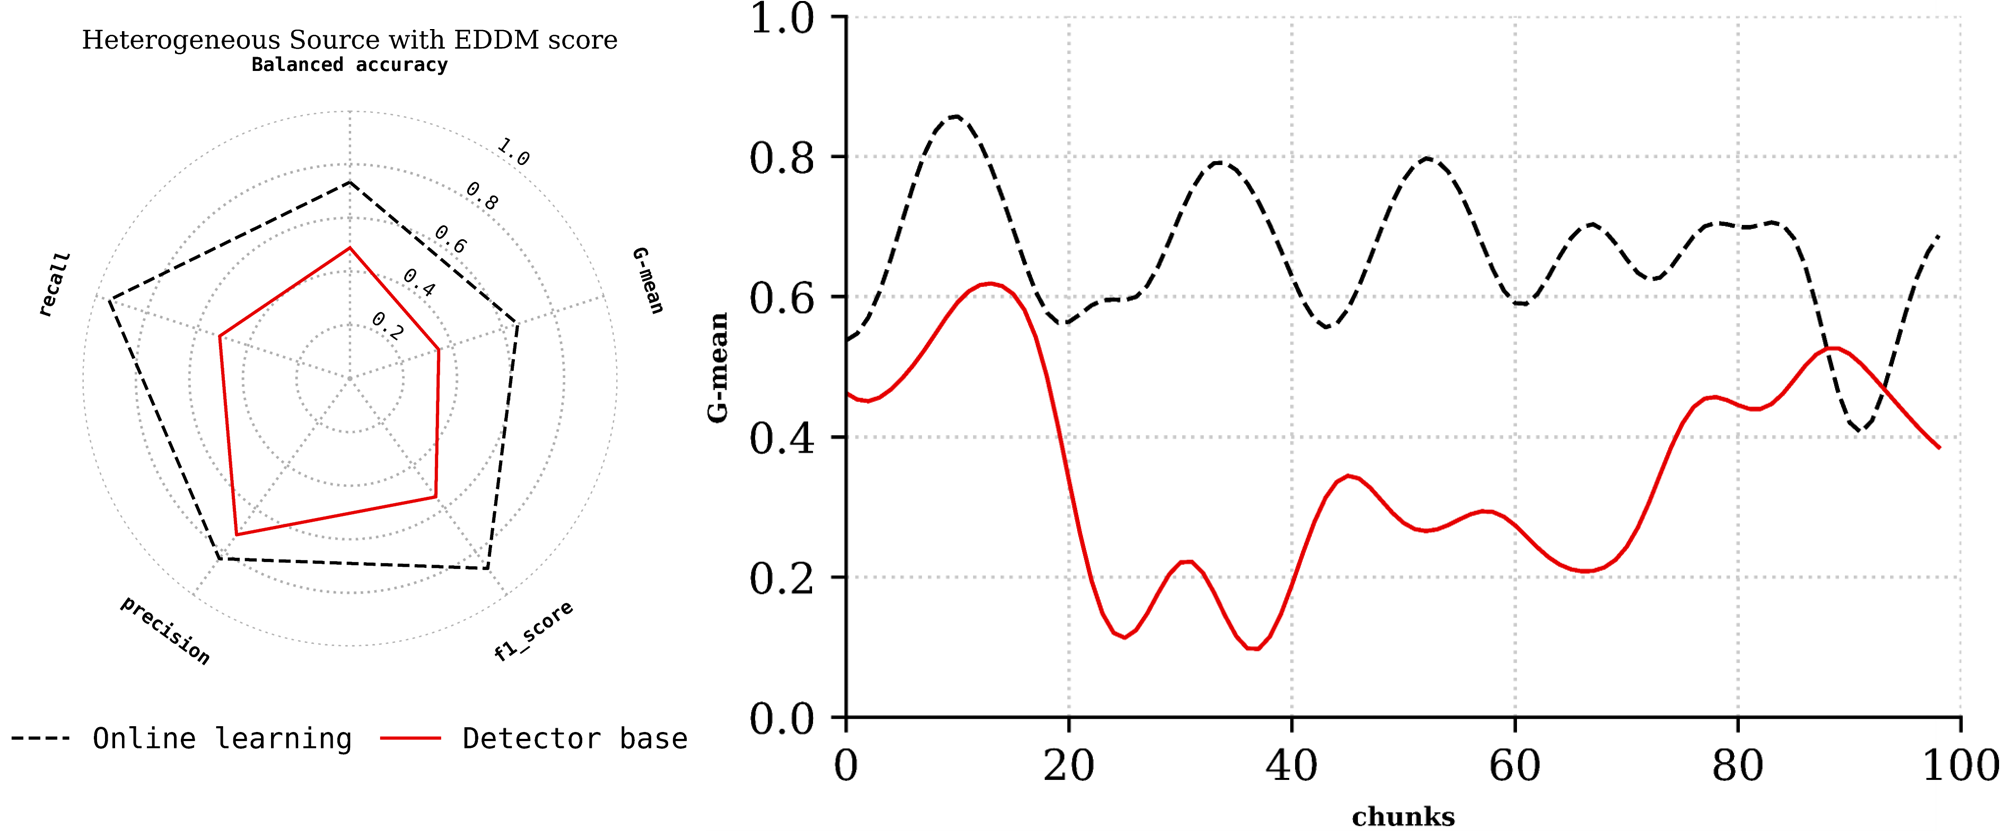
\includegraphics[width=1\linewidth]{6_transfer_learning/figures/exp5.png}
  \caption{Results of online learning and chunk-based detection in the Covertype stream using the ADWIN detector.}
	\label{fig:6_exp7}
\end{figure}
The comparison between online learning, the EDDM detector, and ADWIN reflects a broader philosophical consideration of efficiency, adaptability, and the balance between idealism and practicality. Online learning, with its ability to achieve optimal performance, represents an ideal approach—constantly evolving, adapting to real-time data without reliance on prior knowledge. This continuous adaptation mirrors the notion of becoming, where the system remains in a state of perpetual growth and refinement. The radar diagrams in Figure \ref{fig:6_exp7} further emphasize the superiority of online learning, positioning it as the most effective method. ADWIN, in this context, stands as a favorable compromise, balancing the strengths of online learning with the practicality of reduced time expenditure. ADWIN thus exemplifies the concept of harmony, where competing forces of performance and efficiency are reconciled, offering an adaptable solution that doesn’t strive for perfection but achieves a satisfactory balance. In contrast, the EDDM detector, with its lower performance, reflects the limitations of rigidity—remaining static in the face of evolving data, it fails to respond effectively to dynamic changes. This serves as a reminder of the consequences of inflexibility in systems, where an inability to adapt leads to diminished overall effectiveness. Ultimately, in environments characterized by chunk-based concept drift, especially with the ADWIN detector, the approach that ensures high performance while minimizing computational costs reveals itself as ideal. This balance speaks to the philosophical principle of achieving optimal results through continuous yet measured adaptation \cite{gama2004learning, madkour2023historical}.

\begin{table}[H]
  \centering
  \caption{Runtimes (in seconds) for the Online Learning, ADWIN, and EDMM.}
  \begin{tabular}{|l|c|c|}
  \hline
  \textbf{Technique}       & \textbf{Runtime (in seconds)} & \textbf{Learning Times} \\ \hline
  Online Learning          & 3102             & 100                     \\ \hline
  ADWIN detector           & 2257             & 63                      \\ \hline
  EDMM detector            & 1948             & 40                      \\ \hline
  \end{tabular}
  \label{table:6_table4}
  \end{table}